% =====================================================================
%  Does the Pareto-optimal RAG configuration transfer across GPU tiers?
%  An experiment report.
%  Ahmad Tawil — ahmadtawil.se@gmail.com
%
%  OVERLEAF: upload this file plus figs/fig1.pdf. The bibliography is
%  embedded via filecontents, so no separate .bib upload is needed.
%  Compile: pdfLaTeX -> BibTeX -> pdfLaTeX -> pdfLaTeX.
% =====================================================================

\begin{filecontents*}{refs.bib}
@inproceedings{lewis2020rag,
  author    = {Lewis, Patrick and Perez, Ethan and Piktus, Aleksandra and Petroni, Fabio
               and Karpukhin, Vladimir and Goyal, Naman and K{\"u}ttler, Heinrich
               and Lewis, Mike and Yih, Wen-tau and Rockt{\"a}schel, Tim
               and Riedel, Sebastian and Kiela, Douwe},
  title     = {Retrieval-Augmented Generation for Knowledge-Intensive {NLP} Tasks},
  booktitle = {Advances in Neural Information Processing Systems (NeurIPS)},
  year      = {2020},
  note      = {arXiv:2005.11401}
}
@inproceedings{conway2025syftr,
  author    = {Conway, Alexander and Dey, Debadeepta and Hackmann, Stefan
               and Hausknecht, Matthew and Schmidt, Michael and Steadman, Mark
               and Volynets, Nick},
  title     = {syftr: Pareto-Optimal Generative {AI}},
  booktitle = {International Conference on Automated Machine Learning (AutoML)},
  year      = {2025},
  note      = {arXiv:2505.20266}
}
@article{jiang2025ragstack,
  author  = {Jiang, Wenqi},
  title   = {{RAG-Stack}: Co-Optimizing {RAG} Quality and Performance
             From the Vector Database Perspective},
  journal = {arXiv preprint arXiv:2510.20296},
  year    = {2025}
}
@article{kartal2025ragsmith,
  author  = {Kartal, Mehmet Yasin and Kose, S. K. and Sevin{\c{c}}, K. and Aktas, B.},
  title   = {{RAGSmith}: A Framework for Finding the Optimal Composition of
             Retrieval-Augmented Generation Methods Across Datasets},
  journal = {arXiv preprint arXiv:2511.01386},
  year    = {2025}
}
% VERIFY: venue line (SOSP '25) and author list not independently confirmed.
@inproceedings{ray2025metis,
  author    = {Ray, Siddhant and Pan, Rui and Gu, Zhuohan and Du, Kuntai
               and Feng, Shaoting and Ananthanarayanan, Ganesh
               and Netravali, Ravi and Jiang, Junchen},
  title     = {{METIS}: Fast Quality-Aware {RAG} Systems with Configuration Adaptation},
  booktitle = {Proceedings of the ACM Symposium on Operating Systems Principles (SOSP)},
  year      = {2025},
  note      = {arXiv:2412.10543}
}
@inproceedings{reimers2019sbert,
  author    = {Reimers, Nils and Gurevych, Iryna},
  title     = {{Sentence-BERT}: Sentence Embeddings using Siamese {BERT}-Networks},
  booktitle = {Proceedings of EMNLP-IJCNLP},
  year      = {2019},
  note      = {arXiv:1908.10084}
}
@article{xiao2023cpack,
  author  = {Xiao, Shitao and Liu, Zheng and Zhang, Peitian and Muennighoff, Niklas
             and Lian, Defu and Nie, Jian-Yun},
  title   = {{C-Pack}: Packed Resources For General Chinese Embeddings},
  journal = {arXiv preprint arXiv:2309.07597},
  year    = {2023}
}
@article{douze2024faiss,
  author  = {Douze, Matthijs and Guzhva, Alexandr and Deng, Chengqi and Johnson, Jeff
             and Szilvasy, Gergely and Mazar{\'e}, Pierre-Emmanuel and Lomeli, Maria
             and Hosseini, Lucas and J{\'e}gou, Herv{\'e}},
  title   = {The {Faiss} library},
  journal = {arXiv preprint arXiv:2401.08281},
  year    = {2024}
}
@article{bajaj2016msmarco,
  author  = {Bajaj, Payal and Campos, Daniel and Craswell, Nick and Deng, Li
             and Gao, Jianfeng and Liu, Xiaodong and Majumder, Rangan
             and McNamara, Andrew and Mitra, Bhaskar and Nguyen, Tri
             and Rosenberg, Mir and Song, Xia and Stoica, Alina
             and Tiwary, Saurabh and Wang, Tong},
  title   = {{MS MARCO}: A Human Generated MAchine Reading COmprehension Dataset},
  journal = {arXiv preprint arXiv:1611.09268},
  year    = {2016}
}
@article{qwen2024qwen25,
  author  = {{Qwen Team}},
  title   = {{Qwen2.5} Technical Report},
  journal = {arXiv preprint arXiv:2412.15115},
  year    = {2024}
}
@article{kendall1938,
  author  = {Kendall, M. G.},
  title   = {A New Measure of Rank Correlation},
  journal = {Biometrika},
  volume  = {30}, number = {1--2}, pages = {81--93}, year = {1938},
  doi     = {10.1093/biomet/30.1-2.81}
}
@unpublished{tawil2026david,
  author = {Tawil, Ahmad},
  title  = {David vs Goliath: Agentic versus Naive {RAG} across Model Scales},
  year   = {2026},
  note   = {Unpublished manuscript}
}
\end{filecontents*}

\documentclass[10pt,a4paper]{article}

\usepackage[T1]{fontenc}
\usepackage[utf8]{inputenc}
\usepackage{lmodern}
\usepackage[margin=1in]{geometry}
\usepackage{graphicx}
\usepackage{booktabs}
\usepackage{amsmath}
\usepackage{microtype}
\usepackage{caption}
\usepackage{listings}
\usepackage[numbers,sort&compress]{natbib}
\usepackage[hidelinks,breaklinks]{hyperref}

\newcommand{\hs}[1]{{\small\ttfamily #1}}
\lstset{basicstyle=\footnotesize\ttfamily, frame=single, framesep=3pt,
        breaklines=true, columns=fullflexible,
        xleftmargin=3.4pt, xrightmargin=3.4pt,
        aboveskip=7pt, belowskip=7pt}
\captionsetup{font=small,labelfont=bf}
\setlength{\parskip}{0.3em}

\title{\bfseries Does the Pareto-optimal RAG configuration\\transfer across GPU tiers?\\[4pt]
       \large\normalfont An experiment report}
\author{Ahmad Tawil\\\small\texttt{ahmadtawil.se@gmail.com}}
\date{\today}

\begin{document}
\maketitle

\begin{abstract}
\noindent
Papers that search for good retrieval-augmented generation (RAG) configurations
publish a recommended setup benchmarked on the authors' hardware. Practitioners
copy it onto cheaper cards. This report tests whether the recommendation
survives that move. I ran an identical 96-configuration grid --- chunk size,
overlap, embedding model, top-$k$, reranker --- on an NVIDIA A100-SXM4-40GB and
an NVIDIA L4, against one corpus and one hand-labelled gold set, with every
result record provenance-stamped. Retrieval quality is deterministic and came
out identical on both cards, so every change in the result is attributable to
latency alone. The Pareto frontier is not the same on both: four configurations
on the A100, six on the L4, three shared, with Kendall's $\tau = 0.802$ between
the two latency rankings. The difference survives both latency statistics and an
$\varepsilon$-dominance tolerance of 300\,ms. My pre-registered hypothesis --- that
cross-encoder reranking would flip from optimal to dominated on the weaker card
--- did not hold: reranking appears on both frontiers. The practical
consequence is that copying a published shortlist onto different hardware can
leave you running a configuration that is slower than an equally accurate
alternative, at no visible cost in quality.
\end{abstract}

% ====================================================================
\section{Introduction}
% ====================================================================

Every paper that searches the RAG configuration space ends with a
recommendation: this chunk size, this top-$k$, rerank or do not. That
recommendation is produced once, on whatever GPU the authors had, and then
travels --- into blog posts, into default settings, into production systems
running on hardware an order of magnitude weaker. The move is never validated,
because the experiment that would validate it requires running the same grid
twice on deliberately mismatched hardware, and configuration-search papers are
built to explore the algorithm space rather than the hardware axis. The result
is a literature of optimality claims with an unstated precondition attached.

This report supplies the missing measurement. \textbf{The same 96-configuration
grid, the same corpus, the same hand-labelled gold set and the same code were
executed on two GPU tiers separated by roughly $5.2\times$ in memory
bandwidth}, and both result sets were recorded in full. Three properties make
the comparison worth trusting:

\begin{itemize}\itemsep2pt
  \item \textbf{The hypothesis and its refutation condition were committed to
        version control before the first cell ran}, and neither was edited
        afterwards. The result reported here is the one the experiment was
        designed to be able to contradict.
  \item \textbf{Retrieval quality came out bit-identical across cards}, which
        removes the confound entirely: every difference in the result is a
        latency effect, and nothing else is available to explain it.
  \item \textbf{Every record is self-describing} --- GPU, driver, library
        versions, git SHA, corpus and gold-set hashes --- so no claim here
        depends on external state, and any cell can be regenerated from its
        identifier alone.
\end{itemize}

The question is: \textbf{does the Pareto-optimal RAG configuration transfer
across GPU tiers, or does the ranking of configurations change?}

\paragraph{Hypothesis, registered in advance.}
The Pareto-optimal configuration is not hardware-invariant. Chunk size and
top-$k$ keep their optimal settings, but cross-encoder reranking flips from
Pareto-optimal on the A100 to Pareto-dominated on the L4, because its latency
cost grows faster than the recall it buys.

\paragraph{Refutation condition.} Both frontiers contain the same
configurations in the same order.

\paragraph{Outcome.} The frontiers differ, and the difference is robust to both
the choice of latency statistic and to 300\,ms of assumed host noise. The
mechanism named in the hypothesis did not occur: reranking holds a frontier slot
on both cards. \S\ref{sec:results} reports which claim the evidence supports and
which it does not, and \S\ref{sec:threats} states what would be needed to settle
the remainder.

% ====================================================================
\section{Related work}
% ====================================================================

Multi-objective RAG configuration search is a crowded literature, and this
report does not claim to be first to locate a Pareto frontier over retrieval
configurations. \textbf{syftr}~\citep{conway2025syftr} runs multi-objective
Bayesian optimisation over agentic and non-agentic RAG flows, balancing accuracy
against cost on a single hardware target. \textbf{RAG-Stack}~\citep{jiang2025ragstack}
identifies the quality--performance frontier across the joint algorithm--system
design space, and is the closest prior work to acknowledge hardware at all --- but
it explores from the algorithm side, treating the system as a fixed backdrop.
\textbf{RAGSmith}~\citep{kartal2025ragsmith} runs evolutionary search over
complete pipelines and reports sensitivity to the dataset it was tuned on, which
is adjacent to but distinct from hardware sensitivity.
\textbf{METIS}~\citep{ray2025metis} performs joint algorithm/system exploration,
again on fixed hardware. The underlying RAG approach is due to
\citet{lewis2020rag}.

In all four, the hardware tier is a constant rather than a variable. None asks
whether the configuration it recommends would still be recommended on a smaller
GPU.

\begin{quote}\itshape
Existing work locates the configuration frontier on fixed hardware; whether the
frontier's composition is stable across hardware tiers has not been tested.
\end{quote}

The finding has the same shape as an earlier result of my
own~\citep{tawil2026david}, which found the optimal RAG \emph{strategy} depends
on model scale where this one finds the optimal \emph{configuration} depends on
hardware tier. Both say the same thing about what ``optimal'' means in this
literature: it is conditional on something the recommending paper held fixed.

% ====================================================================
\section{Experimental setup}
\label{sec:setup}
% ====================================================================

\paragraph{Pipeline.} Recursive character chunking $\rightarrow$
\texttt{sentence-transformers} embedding~\citep{reimers2019sbert} $\rightarrow$
FAISS~\citep{douze2024faiss} \texttt{IndexFlatIP} retrieval over
$L_2$-normalised vectors $\rightarrow$ optional cross-encoder rerank
$\rightarrow$ generation. Two BGE embedding models~\citep{xiao2023cpack} are
registered, \texttt{small} (384d) and \texttt{base} (768d), same family so the
contrast is dimension rather than architecture. The reranker is
\texttt{cross-encoder/ms-marco-MiniLM-L6-v2} --- a Sentence-BERT
cross-encoder~\citep{reimers2019sbert} fine-tuned on the MS MARCO passage
ranking data~\citep{bajaj2016msmarco} --- chosen as the lighter of two
candidates specifically because it makes the hypothesis harder to confirm. The
generator is
\texttt{Qwen/Qwen2.5-3B-Instruct}~\citep{qwen2024qwen25}, fixed and unswept:
this is a retrieval-configuration experiment, not a generation-quality one.
Greedy decoding, \texttt{max\_new\_tokens=128}, seed \texttt{1337}, and an
answer-only-from-context prompt (Appendix~\ref{app:setup}).

\paragraph{Corpus and gold set.} 15 PDFs on GenAI/LLM-engineering topics, 72
pages, 35{,}751 tokens, single-subject by design because that retrieves harder
than 15 unrelated documents. 30 questions hand-labelled by one annotator, with
labels recorded as \textbf{character spans in the source document}, never chunk
IDs --- chunk IDs exist only relative to one chunk size, and three of the five
grid knobs change the chunking. A retrieved chunk counts as relevant if it
overlaps a gold span by $\geq 50\%$ of that span. Construction detail, including
the planned question-type distribution and a lexical-saturation problem caught
and fixed during review, is in Appendix~\ref{app:gold}.

\paragraph{Grid.} The first three knobs determine the index; the last two are
query-time only, so 96 cells cost 12 index builds.

\begin{table}[htbp]
\centering\small
\caption{The 96-cell grid. $3\times2\times2 = 12$ indices;
$12\times4\times2 = 96$ cells per card; 192 runs total.}
\label{tab:grid}
\begin{tabular}{@{}llc@{}}
\toprule
Knob & Levels & Count \\
\midrule
Chunk size      & 256 / 512 / 1024 tokens    & 3 \\
Chunk overlap   & 0 / 15\%                   & 2 \\
Embedding model & small (384d) / base (768d) & 2 \\
Top-$k$         & 3 / 5 / 10 / 20            & 4 \\
Reranker        & off / cross-encoder        & 2 \\
\bottomrule
\end{tabular}
\end{table}

\paragraph{Measurement.} Four stages are timed separately --- embed, search,
rerank, generate --- each with \texttt{torch.cuda.synchronize()} before the stop
timestamp, since GPU kernels launch asynchronously and an unsynchronised stop
measures CPU issue rate rather than GPU work. Three warmup queries are
discarded, then each of the 30 gold queries runs three times; $p50$ and $p95$
are computed over all 90 measurements per cell rather than over per-query means.
$p95$ rather than the mean because rented hosts have asymmetric tails. Every
record carries GPU, driver, CUDA, library versions, git SHA, corpus and gold
hashes, and (from the L4 run onward) model revisions. Full harness and
provenance detail is in Appendix~\ref{app:setup}.

\paragraph{Metrics.} \textbf{recall@$k$}: 1 if any top-$k$ chunk is relevant to
any gold span, averaged over 30 queries; reported at $k=5$ (headline) and
$k=10$. \textbf{MRR}: reciprocal rank of the first relevant chunk.
\textbf{Context precision}: fraction of top-5 chunks that are relevant. All
implemented as pure functions and unit-tested against boundary cases including
the recall@$k$ off-by-one at exactly rank $k$.

\paragraph{Hardware.} A100-SXM4-40GB (Ampere, SM80, 40\,GB,
$\sim$1{,}555\,GB/s) and L4 (Ada, SM89, 24\,GB, $\sim$300\,GB/s) --- a bandwidth
ratio of roughly $5.2\times$. The experiment was planned around an A100 80GB
($\sim$2{,}039\,GB/s); the card actually provisioned was the 40GB SKU, confirmed
from the provenance stamp rather than assumed. Software versions per card, and
the reason the two sweeps carry different git SHAs, are in
Appendix~\ref{app:setup}.

% ====================================================================
\section{Results}
\label{sec:results}
% ====================================================================

\paragraph{Retrieval quality is identical across cards.} All 96 recall@5 values
match exactly between the A100 and L4 records. Retrieval is deterministic given
the same index, weights and seed, so the GPU changes speed and nothing else.
Every result below is therefore a latency effect, with no confound from quality.

\paragraph{The frontiers differ.} Seven configurations sit on at least one
card's frontier; the other 89 are dominated on both. The A100 frontier has four
members, the L4 six, and three are shared.

\begin{figure}[htbp]
\centering
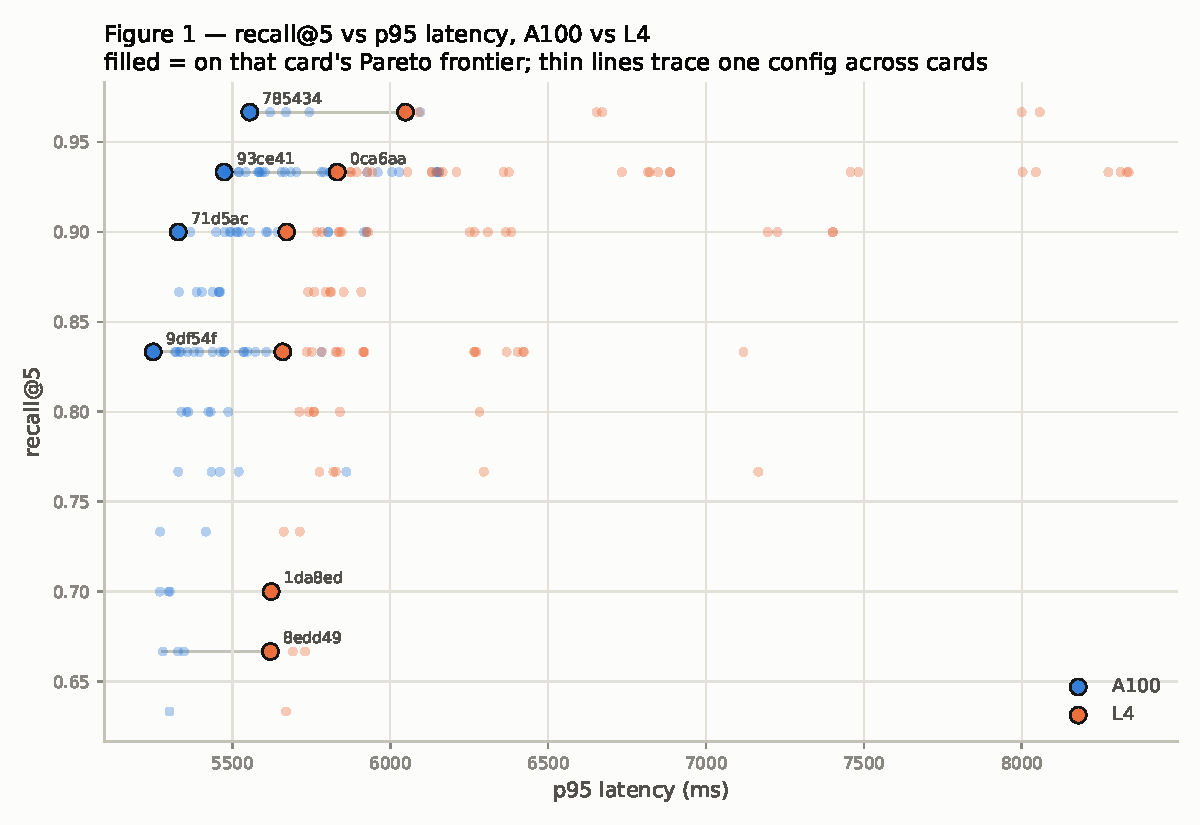
\includegraphics[width=0.95\textwidth]{figs/fig1}
\caption{recall@5 against $p95$ latency for all 96 configurations on both cards.
Ringed points are that card's Pareto frontier; grey lines connect the same
configuration across cards.}
\label{fig:frontier}
\end{figure}

\begin{table}[htbp]
\centering\footnotesize
\caption{Every configuration on at least one frontier. Recall is identical on
both cards, so only latency distinguishes them.}
\label{tab:frontier}
\begin{tabular}{@{}rrlrlrrrl@{}}
\toprule
chunk & ov. & embed & $k$ & reranker & recall@5 & A100 $p95$ & L4 $p95$ & frontier \\
\midrule
256  & 0.0  & base           & 3 & off           & 0.833 & 5249\,ms & 5659\,ms & both \\
256  & 0.0  & base           & 5 & off           & 0.900 & 5329\,ms & 5672\,ms & both \\
1024 & 0.0  & base           & 5 & off           & 0.967 & 5555\,ms & 6048\,ms & both \\
1024 & 0.15 & \textbf{small} & 3 & cross-encoder & 0.933 & 5474\,ms & 5876\,ms & \textbf{A100} \\
1024 & 0.15 & \textbf{base}  & 3 & cross-encoder & 0.933 & 5483\,ms & 5832\,ms & \textbf{L4} \\
256  & 0.0  & small          & 3 & off           & 0.667 & 5280\,ms & 5621\,ms & L4 \\
256  & 0.0  & small          & 3 & cross-encoder & 0.700 & 5298\,ms & 5623\,ms & L4 \\
\bottomrule
\end{tabular}
\end{table}

Kendall's $\tau$~\citep{kendall1938} between the two cards' latency orderings is
$0.802$ over $n=96$: most of the speed ranking transfers, with enough reordering
to produce the difference above. No configuration ran out of memory on either
card, contrary to expectation at
\texttt{chunk=1024}$\times$\texttt{top\_k=20}$\times$cross-encoder.

\paragraph{The reranker did not flip.} Cross-encoder reranking appears on both
frontiers, so the pre-registered mechanism did not occur. Its predicted
economics are nonetheless visible: the rerank stage's latency grows $1.40\times$
from A100 to L4 (ratio of means over the 48 reranker-enabled cells; $1.25\times$
by median of per-cell ratios), against $1.00\times$ for search, $1.04\times$ for
embed and $1.17\times$ for generate. It is the one stage whose cost degrades
disproportionately on the weaker card. It does not decide anything here because
generation dominates: the rerank stage is a median $0.81\%$ of a cell's $p95$
(range $0.32$--$2.16\%$), so the disproportionate slowdown has nowhere large
enough to act. Reranking buys $+0.018$ recall@5 on average, identically on both
cards.

\paragraph{What moved instead.} Two configurations differ only in embedding
model --- rows four and five of Table~\ref{tab:frontier}, both at recall $0.933$
--- and which one holds the frontier slot swaps between cards. The margin is
9\,ms on the A100 and 44\,ms on the L4, under $1\%$ of a $\sim$5{,}800\,ms cell.

\paragraph{How far that survives.} Because those margins are small, the result
was re-derived under two perturbations requiring no new measurement
(Table~\ref{tab:sens}). Varying the latency statistic tests whether the effect is
an artifact of the tail. Widening domination by $\varepsilon$ milliseconds tests
how much host noise it tolerates.

\begin{table}[htbp]
\centering\small
\caption{Frontier composition under both latency statistics and under
$\varepsilon$-dominance on $p95$. Reproducible via
\texttt{scripts/sensitivity.py}.}
\label{tab:sens}
\begin{tabular}{@{}lrrrcc@{}}
\toprule
& A100 & L4 & shared & identical? & embedding swap present? \\
\midrule
$p95$              &  4 &  6 &  3 & no & yes \\
$p50$              &  6 &  7 &  4 & no & \textbf{no} \\
\midrule
$\varepsilon=25$\,ms  & 10 &  9 &  6 & no & --- \\
$\varepsilon=100$\,ms & 29 & 26 & 21 & no & --- \\
$\varepsilon=300$\,ms & 73 & 52 & 52 & no & --- \\
\bottomrule
\end{tabular}
\end{table}

Two claims of different strength follow. \textbf{That the frontiers differ is
robust}: it holds under both statistics and at every $\varepsilon$ up to
300\,ms, roughly seven times the largest deciding margin. \textbf{That the
embedding model is the knob responsible is not}: under $p50$ the frontiers still
differ, but through five other configurations varying in chunk size, top-$k$ and
reranker. The single-knob story is a property of the tail statistic. I report it
as an illustrative case of how a frontier slot changes hands, not as an
established claim about which knob is hardware-sensitive.

% ====================================================================
\section{Threats to validity}
\label{sec:threats}
% ====================================================================

\paragraph{No repeated-sweep variance estimate.} Each of the 192 cells ran once
per card, and only aggregate statistics were retained, so a bootstrap interval
cannot be recovered retrospectively. The $\varepsilon$-analysis above bounds the
noise the broad result tolerates without estimating it, but the 9--44\,ms
embedding-model margin is exactly the scale a shared host's noisy neighbours
could produce. Repeating only the configurations that decide frontier
membership, rather than the full grid, would settle it cheaply.

\paragraph{Three of four A100 model revisions are inferred.} Revision pinning
originally covered only the embedding models, and wrote the pin to a file on
whichever machine loaded first --- a cloud VM, deleted after the sweep. The
\texttt{small} revision survives because its pin file is git-tracked and was
committed before the sweep; \texttt{base}, the reranker and the generator were
reconstructed by resolving \texttt{main} afterwards, valid under the assumption
that each repository was unchanged since its last update (11 months to 2.4 years
before the sweep) and not force-pushed. The reranker is one arm of the
hypothesis, so this matters. The gap is closed from the L4 run onward.

\paragraph{Single annotator, and a constructed query distribution.} One person
built the corpus and wrote all 30 questions, with no second annotator and no
agreement figure. The query set was also built to a planned distribution rather
than sampled from usage: 8 of 30 written to be lexically confusable across
documents, 6 requiring two documents. Both proportions exceed what natural query
traffic would likely produce, and both favour configurations that rerank and
retrieve at higher $k$. Absolute recall is therefore not comparable to other
corpora; only the relative ordering within this experiment is.

\paragraph{Lexical saturation was mitigated, not eliminated.} A question phrased
in its own answer span's vocabulary is retrievable at any configuration, which
would collapse both frontiers for a reason unrelated to hardware. Five such
questions were caught and rewritten (Appendix~\ref{app:gold}), but that review
had no independent check behind it.

\paragraph{Two cards, one corpus, one embedding family.} The hardware axis has
two points, so this shows that composition changed between these tiers, not how
it changes with GPU class in general --- a gradual shift and a threshold effect
would look identical here. Both embedding models are \texttt{BAAI/bge-*-en-v1.5},
so the sensitivity measured is to embedding \emph{size} within one family.

\paragraph{Single seed.} Fixed at \texttt{1337} and not varied. Narrower than it
appears: decoding is greedy and retrieval is seed-independent, so the three
repeats measure timing rather than generation variance.

% ====================================================================
\section{Conclusion}
% ====================================================================

\textbf{Tested.} One RAG pipeline, 96 configurations, two GPU tiers, identical
corpus, gold set, code and model weights.

\textbf{Found.} Frontier membership differs --- four winners on the A100, six on
the L4, three shared --- and the difference survives both latency statistics and
a 300\,ms domination tolerance. The reranker, which the hypothesis named, did not
change status.

\textbf{Consequence.} Do not assume a published RAG configuration shortlist
transfers unchanged to cheaper hardware. The cost of getting it wrong is not
accuracy --- accuracy is identical --- but latency you did not need to spend, on
a configuration an equally accurate alternative would have beaten. That loss is
invisible unless you measure it.

This experiment does not identify which knob to watch, and \S\ref{sec:results}
is explicit that the candidate it found does not survive a change of statistic.
The defensible advice is about margins rather than knobs: any near-tied pair on a
frontier is a hardware-transfer risk, so re-run the top few candidates on the
deployment card rather than trusting the single published winner.

\appendix

% ====================================================================
\section{Setup detail}
\label{app:setup}
% ====================================================================

\paragraph{Prompt.}
\begin{lstlisting}
Answer the question using ONLY the context below. If the context does not
contain the answer, reply exactly: "I don't know based on the provided context."

Context:
{context}

Question: {question}

Answer:
\end{lstlisting}

\paragraph{Chunking.} Separators are tried coarse-to-fine --- paragraph break,
line break, sentence, word, raw character --- descending into a piece only while
it is over budget. Overlap carries trailing atoms from one chunk into the next
rather than re-slicing. Every chunk retains
\texttt{\{doc\_id, char\_start, char\_end\}} relative to its document's extracted
text, which is what allows span-based gold labels to survive a change of chunk
size.

\paragraph{Model revisions.}

\begin{table}[htbp]
\centering\small
\begin{tabular}{@{}llll@{}}
\toprule
Role & Model & Revision & Provenance \\
\midrule
small     & \texttt{BAAI/bge-small-en-v1.5} & \hs{5c38ec7c\ldots} & measured \\
base      & \texttt{BAAI/bge-base-en-v1.5}  & \hs{a5beb1e3\ldots} & inferred \\
reranker  & \texttt{ms-marco-MiniLM-L6-v2}  & \hs{c5ee24cb\ldots} & inferred \\
generator & \texttt{Qwen2.5-3B-Instruct}    & \hs{aa8e7253\ldots} & inferred \\
\bottomrule
\end{tabular}
\end{table}

``Measured'' means the revision is recorded in a git-tracked file at the commit
stamped on the sweep's records. ``Inferred'' means it was reconstructed
afterwards; see \S\ref{sec:threats}.

\paragraph{Software and hashes.}

\begin{table}[htbp]
\centering\small
\begin{tabular}{@{}lll@{}}
\toprule
 & A100 & L4 \\
\midrule
Driver        & \texttt{580.82.07}    & \texttt{580.82.07} \\
CUDA          & \texttt{12.8}         & \texttt{13.0} \\
\texttt{torch}& \texttt{2.11.0+cu128} & \texttt{2.13.0+cu130} \\
\texttt{sentence-transformers} & \texttt{5.6.0} & \texttt{5.6.1} \\
FAISS         & \texttt{1.14.3}       & \texttt{1.14.3} \\
\texttt{git\_sha} & \hs{04caf49}      & \hs{3761de1} \\
\bottomrule
\end{tabular}
\end{table}

Both content hashes are identical on all 192 records:

\begin{table}[htbp]
\centering\small
\begin{tabular}{@{}ll@{}}
\toprule
\texttt{corpus\_sha} & \hs{a2a9aecc051466d25ff4f3e48aaf2c69aba1a8aa} \\
\texttt{gold\_sha}   & \hs{3afa042d8d9cd6784e8e1b049e4f4f6c1d45709c} \\
\bottomrule
\end{tabular}
\end{table}

The two sweeps carry different \texttt{git\_sha} values because the
revision-pinning fix landed between them. The difference is provenance capture
only: every file the retrieval and generation path executes is byte-identical
between the two commits except two import statements from a package
restructure.

\paragraph{Other harness details.} Peak VRAM is the high-water mark across a
cell (\texttt{reset\_peak\_memory\_stats} then \texttt{max\_memory\_allocated}).
An out-of-memory cell is caught and written with \texttt{status="oom"} and no
cost or quality block rather than crashing the sweep or being skipped; such a
cell cannot be a frontier member by construction, and is reported in a refusals
table. Indices are cached on
\texttt{(chunk\_size, overlap, embed\_model)} so the sweep rebuilds 12 times
rather than 96. Any single cell regenerates from its \texttt{config\_id} with one
command.

% ====================================================================
\section{Gold set construction}
\label{app:gold}
% ====================================================================

Question types were allocated before any question was written: 7 with
single-sentence answers, 9 with paragraph answers, 8 lexically confusable across
documents, 6 requiring two documents. That yields 30 questions and 38 gold
spans, covering all 15 documents, with span lengths from 38 to 414 characters
(median 193).

Spans were located against the same \texttt{pypdf}-extracted text the pipeline
indexes, not the PDF's visual layout, using a helper that returns exact offsets
so none were hand-counted. Thirteen initially-quoted spans did not resolve on
the first pass, because code listings extract with line numbers interleaved,
identifiers extract letter-spaced, and some punctuation swallows adjacent
spaces. All were re-resolved and verified before the gold set was hashed and
frozen.

Two review passes were run. The first found two mislabelled
confusable-document pairs, corrected, and five questions with high content-word
overlap against their own gold span (47--62\%; one reused six of the span's
terms in the span's order). A question phrased in its answer's vocabulary is
retrievable by near-lexical match regardless of configuration --- recall
saturates across the grid, both cards produce identical frontiers, and the
result reads as a transfer finding when it is really a dead instrument. All five
were rewritten to describe the answer without its source terminology, targeting
the same spans.

\bibliographystyle{plainnat}
\bibliography{refs}

\end{document}
